\chapter{O algoritmo de homotopia}

O algoritmo de Homotopia é um algoritmo com o objetivo de resolver $\eqref{eqn:P1}$ minimizando funções do tipo
$$J_{\lambda_n}(x) = \frac{1}{2} \Vert Ax - y \Vert_2^2 + \lambda_n \Vert x \Vert_1$$
para uma sequência decrescente $(\lambda_n)$ de números positivos.

Podemos encontrar o mínimo de uma função diferencial $f: \mathbb{R}^n \longrightarrow \mathbb{R}$ procurando os pontos $x$ no domínio em que $\nabla f(x) = 0$. No nosso caso, a norma $1$ não é diferenciável. Então será definida uma generalização para a diferencial, que será usada no algoritmo, chamado de Homotopia.

\begin{definicao}
Seja $f: \mathbb{R}^n \longrightarrow \mathbb{R}$. A subdiferencial de $f$ em $x \in \mathbb{R}$ é dada por

$$\partial f(x) = \{ v \in \mathbb{R}^N : f(y) - f(x) \geq \langle v, y - x \rangle, \forall y \in \mathbb{R}^N \}$$

%Mostrar que a subdiferencial é uma generalização da diferencial
% >>> http://www.staff.science.uu.nl/~balde101/cao10/cursus10_1.pdf
\end{definicao}

Não é difícil ver que o operador $\partial$ é linear. A subdiferencial coincide com a diferencial de uma função, quando ela for convexa e diferenciável, como mostra a seguinte proposição:

\begin{proposicao}
Se $f: \mathbb{R}^n \longrightarrow \mathbb{R}$ for convexa e diferenciável, então para todo $x \in \mathbb{R}^n$, $\partial f(x) = \{ \nabla f(x) \}$.
\end{proposicao}
%\begin{proof}
%Dados $x, y \in \mathbb{R}^n$, defina a seguinte curva $\gamma: \left[0,1\right]$.
%\end{proof}

Um ponto $x_0$ é ponto de mínimo de uma função $f$ se, e somente se, $0 \in \partial f$, pois
$$ \forall x \in \mathbb{R}^n, f(x) - f(x_0) \geq 0 = \langle 0, x - x_0 \rangle$$.

%Explicar melhor, por exemplo, dizer que \partial (v1, v2) = \partial v1 \times \partial v2
Como a norma $1$ é convexa, sua subdiferencial em um ponto $x$ é um vetor $v$ tal que para cada $i = 1, \hdots, n$,
$$ v_i =
\begin{cases}
	sgn(v_i) & \mbox{ se } v_i \neq 0 \\
	\lbrace 1, -1\rbrace & \mbox{ se } v_i = 0
\end{cases}$$
%Citar FornasireFinal_red.pdf, que definiu a subdiferencial de f

%@inproceedings{yang2010fast,
%  title={Fast ℓ 1-minimization algorithms and an application in robust face recognition: A review},
%  author={Yang, Allen Y and Sastry, S Shankar and Ganesh, Arvind and Ma, Yi},
%  booktitle={2010 IEEE International Conference on Image Processing},
%  pages={1849--1852},
%  year={2010},
%  organization={IEEE}
%}

O algoritmo de Homotopia \cite{fornasier} \cite{dontsa} minimiza a função em um número finito de passos. Fixado um $\lambda$ positivo, considere a seguinte função :

$$J_{\lambda} (x) = \frac{1}{2} \Vert Ax - y \Vert_2^2 + \lambda \Vert x \Vert_1$$

%citar quem mostra que a curva é linear por partes
e seu respectivo minimizador $x_\lambda$. Quando $\lambda$ é grande, $x_{\lambda} = 0$. O ponto $\tilde{x}$, solução de $\eqref{eqn:P1}$ é solução de algum $J_{\tilde{\lambda}}$. A curva $\lambda \longmapsto x_{\lambda}$ é linear por partes, então é possível encontrar a solução de $\eqref{eqn:P1}$ com um número finito de passos.

A subdiferencial de $J_\lambda$ é

$$\partial J_\lambda(x) = A^{T}(Ax - y) + \lambda \partial \Vert x \Vert_1$$

Se $x = x_\lambda$ então $0 \in \partial J_\lambda(x)$ é equivalente a

\begin{equation}
\begin{cases}
(A^*(Ax - y))_i           =    \lambda sgn(x_i), &\mbox{se } x_i \neq 0\\
\vert A^*(Ax - y)\vert_i  \leq \lambda,          &\mbox{se } x_i = 0
\end{cases}
\label{eqn:hom0}
\end{equation}

para $i \in \{1, \hdots, n \}$, onde $sgn(x_i) = 1$ se $x_i \geq 0$ e $0$ caso contrário.

Escrevendo $c = A^{T}(Ax - y)$ e denotando $I$ como o suporte de $x$, então $\eqref{eqn:hom0}$ equivale a

\begin{equation}
\begin{cases}
c(I)           =    \lambda sgn(x_{\lambda}(I)) \\
\vert c(I^{\texttt{c}}) \vert \leq \lambda
\end{cases}
\label{eqn:hom1}
\end{equation}

O algoritmo de Homotopia procura os vértices da curva $\lambda \longmapsto x_\lambda$. Começando com $x_0 = 0$, em uma iteração $l$, $\lambda_l = \Vert c(I) \Vert_{\infty}$, com $I$ denotando o suporte de $x_l$. Depois, o algoritmo calcula uma direção $d_l$, onde

\begin{equation}
\begin{cases}
A^{\texttt{T}}_I A_I d_l(I) = sgn (c_l(I)) \\
d_l(I^{\texttt{c}}) = 0
\end{cases}
\label{eqn:hom2}
\end{equation}

$A_I$ denota a matriz $\left[A_{i_1}, \hdots, A_{i_r}\right]$, onde cada $i_r \in I$ e cada $A_{i_r}$ é uma $i_r$-ésima coluna de $A$. Da mesma maneira, $d_l(I)$ é o vetor calculado após remover todos os elementos de $d_l(i)$ tais que $i \notin I$.

A magnitude $\gamma_l$ do passo $d_l$ é calculada como o menor valor em que a equação $\eqref{eqn:hom1}$ não seja mais válida, ou seja, para $x_{l+1} = x_{l} + \gamma_l d_l$, teremos que pelo menos uma das seguintes condições será satisfeita:

\begin{enumerate}[(i)]
\item para algum $i \in I, \vert (c_l)_i \vert \ > \lambda$. Isso ocorre para $\gamma_l = \gamma_l^{+}$, onde
$$ \gamma_l^{+} = \min_{i \in I^c} \left\lbrace \frac{\lambda_l - c_l(i)}{1 - a_i^T v_l}, \frac{\lambda_l + c_l(i)}{1 + a_i^T v_l} \right\rbrace$$

Onde $v_l = A_I d_l(I)$.

\item para algum $i \in I, (x_{l+1})_i = 0$, o que equivale a $\gamma = \gamma^{-}$, onde
$$ \gamma_l^{-} = \min_{i \in I} \left\lbrace \frac{- x_l(i)}{d_l(i)} \right\rbrace$$
\end{enumerate}

Então calculamos $\gamma = \min \lbrace \gamma_l^{-}, \gamma_l^{+} \rbrace$. O algoritmo termina quando $c_l = 0$ ou quando $ \lambda_{l} = \Vert c_{l} \Vert_{\infty} \leq \lambda_{l - 1} = \Vert c_{l - 1} \Vert_{\infty}$

O Algoritmo $\ref{alg:homotopia}$ mostra o funcionamento passo a passo.

%ver http://www.cs.toronto.edu/~frank/Useful/algorithm2e.pdf
\begin{algorithm}[H]
%	\SetAlgoLined
	\Entrada{$A$ matriz $m \times n$, $y \in \mathbb{R}^m$}
	\Saida{$x \in \mathbb{R}^n$ esparso com $Ax = y$}
	\Inicio{
		$\lambda_{0} = -1$ \\
		$l = 1$  \\
		$x_l = 0$, $c_l = -A^Ty$, $\lambda_l = \Vert c_l \Vert_{\infty}$ \\
		$I = supp ( c_l )$\\
		\Enqto{$\lambda_l \geq 0$ e $\lambda_l > \lambda_{l - 1}$}{
			$d_l = (A_I^TA_I)^{\dagger} sgn(c_l(I)) = A_I^{\dagger} (A_I^{\dagger})^T sgn(c_l(I))$\\
			$v_l = A_I d_l(I)$ \\
			Calcular $\gamma_l^{+}$ como o valor mínimo da família
			$\lbrace \frac{\lambda_l - c_l(i)}{1 - a_i^Tv_l} \rbrace_{i \in I^c}$
			e $i^{+}$ o índice onde esse valor é atingido.\\
			
			Calcular $\gamma_l^{-}$ como o valor mínimo da família
			$\lbrace \frac{-x_l(i)}{d_l(i)} \rbrace_{i \in I}$
			e $i^{-}$ o índice onde esse valor é atingido.\\
			
			$\lambda_l = \min\lbrace\lambda_l^{-}, \lambda_l^{+}\rbrace$ \\
			$i = \min \lbrace i^{-}, i^{+} \rbrace$\\
			
			\eSe{$i \in I$}{Adicionar $i$ a $I$}{Remover $i$ de $I$}
			
			$x_{l+1} = x_l + \lambda_ld_l$ \\
			$l = l + 1$\\
			$c_l = A^T(Ax_l - y)$	
		}
	}
	\label{alg:homotopia}
	\caption{Homotopia}
\end{algorithm}

Como o programa calcula a pseudoinversa de $A_I$ em cada iteração e entre uma iteração e a seguinte $A_I$ tem uma coluna a mais ou a menos que a $A_I$ anterior, fizemos uma adaptação do algoritmo recursivo de pseudoinversa \cite{greville1958pseudoinverse} para calcular de maneira mais eficiente$A_I^{\dagger}$ quando adicionamos um elemento a $I$, a pseudoinversa anterior.

Quando removemos um elemento de $I$, calculamos $A_I^{\dagger}$ da maneira usual.
\section{Exemplo}

Usamos o algoritmo de homotopia para recuperar uma imagem usando diferentes taxas de compressão.

Fixada uma taxa de compressão $r$, calculamos $m = r \cdot n$. Dada uma imagem, calculamos um frame com a transformada do cosseno da imagem e depois obtemos um vetor $x$ empilhando todas as colunas do frame. Em seguida, calculamos $y = Ax$, onde os elementos de $A$ são iid $\mathcal{N}(0,1)$. Depois encontramos uma aproximação $\tilde{x}$ para $x$ usando o algoritmo de homotopia.

A Figura $\ref{fig:homotopy}$ mostra imagens recuperadas pelo algoritmo de homotopia usando diferentes taxas de compressão e mostra também uma imagem recuparada usando o método de mínimos quadrados (MMQ). Note que, para taxas de compressão de $40\%$ e $80\%$, o algoritmo de homotopia apresenta melhor resultado que o algoritmo MMQ com $r = 80\%$.

\begin{figure}
\centering
	\begin{subfigure}[b]{0.4\textwidth}
        \centering
        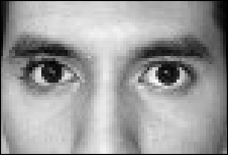
\includegraphics[scale=1]{imagens/homotopy/original.png}
        \caption{imagem original}
	    \label{fig:homotopy_original}
    \end{subfigure}
    ~
    \begin{subfigure}[b]{0.4\textwidth}
        \centering
        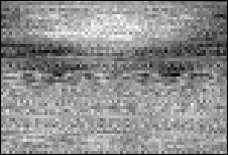
\includegraphics[scale=1]{imagens/homotopy/80porcento.png}
        \caption{compressão de $80\%$}
	    \label{fig:homotopy_20porc}
    \end{subfigure}\\    
    \begin{subfigure}[b]{0.4\textwidth}
        \centering
        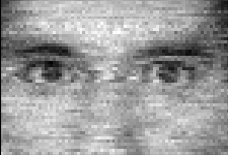
\includegraphics[scale=1]{imagens/homotopy/40porcento.png}
        \caption{compressão de $40\%$}
	    \label{fig:homotopy_40porc}
    \end{subfigure}
    ~
    \begin{subfigure}[b]{0.4\textwidth}
        \centering
        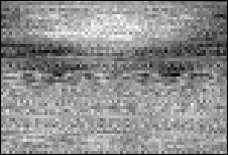
\includegraphics[scale=1]{imagens/homotopy/20porcento.png}
        \caption{compressão de $20\%$}
	    \label{fig:homotopy_80porc}
    \end{subfigure}\\
    \begin{subfigure}[b]{0.4\textwidth}
        \centering
        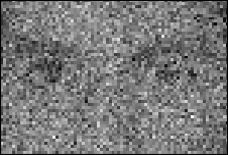
\includegraphics[scale=1]{imagens/homotopy/80porcentoMMQ.png}
        \caption{Imagem recuperada usando o método de mínimos quadrados com compressão de $80\%$}
	    \label{fig:MMQ_80porc}
    \end{subfigure}\\
    \caption{{\bf (a)} Imagem original; {\bf (b)}, {\bf(c)} e {\bf (d)} Imagens recuperadas com o algoritmo de homotopia usando diferentes taxas de compressão; {\bf (e)} Imagem recuperada usando o método de mínimos quadrados.}
    \label{fig:homotopy}
\end{figure}